%template for producing IEEE-format articles using LaTex.
%written by Matthew Ward, CS Department, Worcester Polytechnic Institute. 
%use at your own risk. Complaints to /dev/null.
%make two column with no page numbering, default is 10-point 
\documentstyle[twocolumn,psfig]{article}
\pagestyle{empty}
%set dimensions of columns, gap between columns, and paragraph indent 
\setlength{\textheight}{8.75in}
\setlength{\columnsep}{2.0pc}
\setlength{\textwidth}{6.8in}
\setlength{\footheight}{0.0in}
\setlength{\topmargin}{0.0in}
\setlength{\headheight}{0.0in}
\setlength{\headsep}{0.0in}
\setlength{\oddsidemargin}{-.19in}
\setlength{\parindent}{1pc}
%I copied stuff out of art10.sty and modified them to conform to IEEE format
\makeatletter
%as Latex considers descenders in its calculation of interline spacing,
%to get 12 point spacing for normalsize text, must set it to 10 points 
\def\@normalsize{\@setsize\normalsize{10pt}\xpt\@xpt
\abovedisplayskip 10pt plus2pt minus5pt\belowdisplayskip 
\abovedisplayskip \abovedisplayshortskip \z@ 
plus3pt\belowdisplayshortskip 6pt plus3pt 
minus3pt\let\@listi\@listI}
%need an 11 pt font size for subsection and abstract headings 
\def\subsize{\@setsize\subsize{12pt}\xipt\@xipt}
%make section titles bold and 12 point, 2 blank lines before, 1 after 
\def\section{\@startsection {section}{1}{\z@}{1.0ex plus 1ex minus .2ex}{.2ex plus .2ex}{\large\bf}}
%make subsection titles bold and 11 point, 1 blank line  before, 1 after 
\def\subsection{\@startsection {subsection}{2}{\z@}{.2ex plus 1ex} {.2ex plus .2ex}{\subsize\bf}}
\makeatother

\begin{document}
%don't want date printed
\date{}
%make title bold and 14 pt font (Latex default is non-bold, 16pt) 
\title{\Large\bf Who Limits the Parallelism of Multithreaded Programs}
%for single author (just remove % characters)
%\author{I. M. Author \\
%  My Department \\
%  My Institute \\
%  My City, STATE, zip}
%for two authors (this is what is printed) 
\author{\begin{tabular}[t]{c@{\extracolsep{8em}}c} 
Huayang Guo  & Gang Hu \\
 \\
        Computer Science & Computer Science \\
        Columbia University & Columbia University \\
        New York, NY, 10027 & New York, NY, 10027 \\
        huayang@cs.columbia.edu & ganghu@cs.columbia.edu
\end{tabular}}
\maketitle
%I don't know why I have to reset thispagestyle, but otherwise get page numbers 

\thispagestyle{empty}
\subsection*{\centering Abstract}
%IEEE allows italicized abstract
{\em

DRAFT: Parallelism of software programs is influenced by many factors 
including code quality, underlying infrastructure, I/O bandwidth, and,
maybe VMM. In this report, we tend to evaluate the influence of VMM on 
modern multi-threaded programs and diagnose potential issues that limit 
the parallelism on virtual machines. 

palapala

%end italics mode
}



\section{Introduction}

It has been a hot research direction of parallelism in the recent two or 
three decades. A bunch of frameworks are invented to help programmers 
write better parallelized, more reliable and clearer codes. OpenMP, MPI, 
POSIX thread libraries, and big vendors like MapReduce, Amazon EC2 have made
it extremely easy and common to write a parallel program. 

There has always been, however, a gap between research work and practical 
multithreaded programs. Silas pointed out in 2010 that a great number of 
multithreaded programs will reach parallelization bottleneck when the 
number of cores scale up. For example, \emph{memcached}, a popular in 
memory cache program, scales poorly (as showed in figure 
\ref{figure:memcached})
by the number of cores on Linux 
operating system, even if the codes is very carefully written. The main 
reason of this bottleneck is a piece of kernel codes leads to significant 
overhead in kernel time, which limits the parallelism of \emph{memcached}.
\begin{figure}[H]
\center
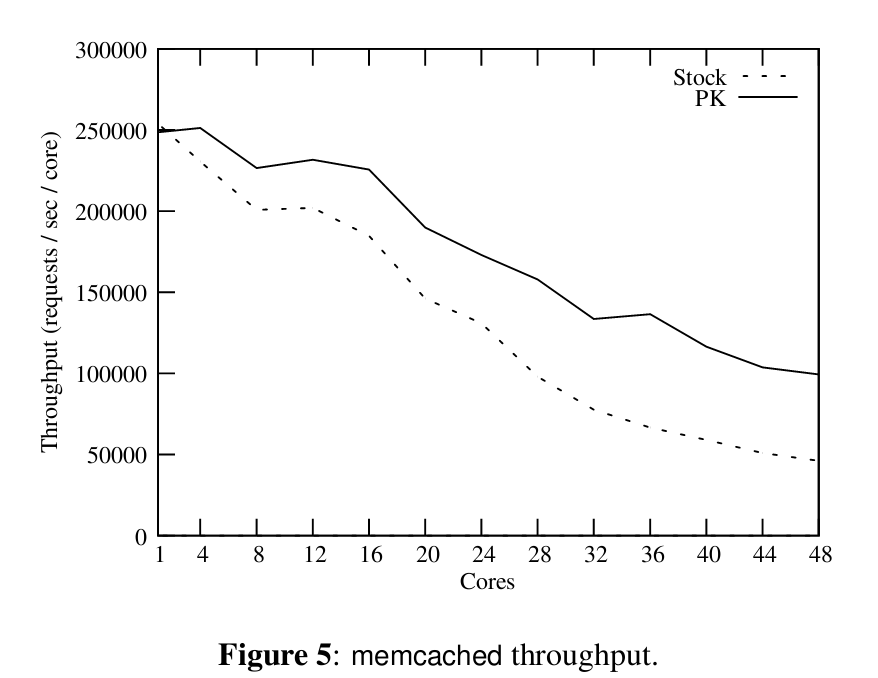
\includegraphics[width=0.8\linewidth]{figures/memcachced_scal.png}
\caption{Parallelism bottleneck of \emph{memcached} on Linux} 
\label{figure:memcached}
\end{figure}
Operating system kernel is one external factor that might limit the 
parallelism of our programs, but definitely not the only one. I/O speed, 
network condition, hardware configuration, scheduling algorithm and many
more might change the scalability curve or multithreaded programs. 

In this project, we target the influence of virtual machines/emulators on 
the parallelism of multithreaded programs. Here're some reasons why we choose
VM/emulator for study.
\begin{itemize}
\item Vritualization techniques abstracts the hardware from operating system 
and enables multiple operating systems running on shared hardware resources
simutaneously. It's very important to schedule the resources between different
guest OS to keep all fast and alive. To achieve this goal, improve program 
parallelism to use hardware computing power exaustively is necessary.
\item It has been only a short time from VMs/emulators start to support multicore
systems. Developers and researchers might not be able to do careful study 
on parallelism support of general mulithreaded programs. Even today some 
CPU architectures are not well supported for multiprocessor virtualization.
\begin{table}
\center
\begin{tabular}{c|c}
Virtual Machine/Emulator & Support parallelization from \\
\hline
QEMU & 2010\cite{rel:qemuwiki} \\
VMWare & 2008\cite{rel:vm55} \\
Xen & 2005\cite{rel:xenpar}\cite{rel:xen} 
\end{tabular}
\end{table}
\item VMs/emulators have to control the schedule of CPU slices 
without careful consideration of what's running on the guest machine. 
\item Many VMs/emulators are open-source.
\end{itemize}

After considering both history and simplicity, we selected QEMU for our 
experiment purpure. QEMU is a used as a system emulator to run popular 
multithreaded benchmarks
(splash2, REDIS), as well as some dedicated microbenchmarks. Hereby we evalute 
specific parallelization properties. Here're briefly our results. 

\begin{enumerate}
\item QEMU causes significantly runtime slowdown (approximately 20 times) of all
the benchmarks.
\item QEMU limits the parallelism of some CPU-intensive benchmarks (FFT)
\item QEMU does not have notable scalability issue for any particular kind of 
synchronization operations. 
\end{enumerate}

\paragraph{Roadmap} First, we will show some related works in section 
\ref{sec:rel}. In section \ref{sec:setup}, we will describe the setup of 
our evaluation system and benchmarks. Then in section \ref{sec:res}, we will 
show the result obtained in the experiments. With the results, we wrote some 
dedicated micro-benchmarks and evaluted scalability of synchronizaion operations
in section \ref{sec:mic}.


\section{Related Work}
\label{sec:rel}

\paragraph{Linux Kernel Scalability} Operating system kernel schedules the
execution of multithreaded programs and handles I/O requests for 
applicaitons. Silas\cite{rel:silas} suggested in his paper that potential
careless code in kernel code could significantly limit the parallelism of 
multithreaded programs. They have studied the scalability of some popular 
parallel applications on Linux Kernel and pointed out some issues that 
limit parallelism.
\begin{center}
\begin{tabular}[t] {l|l} 
Application & Bottleneck \\
\hline
Exim &App: Contention on spool directories \\
memcached &HW: Transmit queues on NIC \\
Apache &HW: Receive queues on NIC \\
PostgreSQL &App: Application-level spin lock \\
gmake &App: Serial stages and stragglers \\
pedsort &HW: Cache capacity \\
Metis &HW: DRAM throughpu 
\end{tabular}
\end{center}

\paragraph{Sigificant Overhead in Multicore Virtualization} HiuShan 
\cite{rel:hiushan} addressed the significant overhead of multicore support
in virtual machines in his thesis. Hiushan choose VMWare as the target VM
where Oracle is carefully evaluted for many different operatings on some 
configurations of cores. In the end HiuShan reached the conclusion that VMWare
caused degradation of Oracle parallelism. 

%In subsections there is 1 blank line before the section 
%heading and one afterwards.  Heading text is 11 point 
%bold font.  Paragraphs are indented one pica.  There is 
%no blank line between paragraphs.
%Throughout I may cite references of the form 
%\cite{key:foo} or \cite{foo:baz}, and LaTeX will keep 
%track of numbering.  The numbers are based on the order 
%you place them in the bibliography, not the order they 
%appear in the text.  They should (I believe) be in 
%alphabetical order.  LaTex will put square brackets about 
%the number within the text of your paper.  For those of 
%you new to the bibliography package, you may have to run 
%the latex process twice to allow all references to be 
%resolved. You will get a warning about a missing .aux 
%file.  Just rerun latex and it will be ok.
%


%this is how to do an unnumbered subsection
\section{Discussion}

\paragraph{FFT Scalability Degeneration} Recall the scalability degeneration of FFT
we have seen in figure ~\ref{fig:splash2_vm} and ~\ref{fig:splash2_native}. This 
cannot be explained by extra overhead caused by synchronization operations across
threads, as proved in the microbenchmarks. For future research purpose, we suspect
this is caused by implementation of COREMU. First, COREMU doesn't directly emulate
logic cores on different physical cores but sets up logic cores as kernel threads 
and leaves the scheduling to the host OS kernel. Because the host OS kernel has 
no knowledge of guest OS processes, it cannot make any optimizations to cache line
or data locality. Second, COREMU changes the implementation of system clock, which
might influence the scheduling of guest OS kernel and applications.

\paragraph{QEMU Paralleliation} QEMU emulator applies binary translation on a large
part of emulation and introduces notable overhead for this. The parallelization
implementation, COREMU, however introduces more overhead. COREMU consumes 3 
processors when the guest OS is free and $3 + x$ processors where $x$ is the 
number of virtual cores in guest OS. Another parallelization approach, 
\emph{PQEMU}, which claims better performance of emulation, might be an alternative
choice for the scalability evalutaion. 

\section{Conclusion}
Parallel programs are playing a critical role in state of the art of computing,
so that it's important to narrow the gap between a carefully optimized code and 
a highly parallelized process. In this report, we studied the influence of 
QEMU on program's parallelism. Based on the evaluation on SPLASH-2, REDIS and 
carefully designed microbenchmarks we reached the conclusion that QEMU incurs
parallelism bottleneck for particular programs but scales well for any basic
synchronization operations.


\subsection*{Acknowledgments}
This is how to do an unnumbered subsection, which comes 
out in 11 point bold font.  Here I thank my colleagues, 
especially Mike Gennert, who know more about Tex and 
Latex than I.




\begin{thebibliography}{9}
\bibitem{key:foo}
I. M. Author,
``Some Related Article I Wrote,''
{\em Some Fine Journal}, Vol. 17, pp. 1-100, 1987.
\bibitem{foo:baz}
A. N. Expert,
{\em A Book He Wrote,}
His Publisher, 1989.
\end{thebibliography}



\end{document}


